%% Preamble %%
\documentclass[paper=a4]{article}

\usepackage{float}
\usepackage{geometry}
\geometry{verbose,tmargin=2.25cm,bmargin=2cm,lmargin=2.25cm,rmargin=2cm}
\geometry{a4paper}
\usepackage{multirow}


\usepackage[T1]{fontenc}
\usepackage{fourier}
\usepackage[utf8]{inputenc}
\usepackage[spanish]{babel}				

\usepackage{amsmath,amsfonts,amsthm} % Math packages
\usepackage[pdftex]{graphicx}	

\makeatletter
%%%%%%%%%%%%%%%%%%%%%%%%%%%%%% User specified LaTeX commands.
\usepackage{fancyhdr}
\usepackage{lscape}
\pagestyle{fancy}
\lhead{Electr\'onica II 22.12}
\chead{TPL1}
\rhead{ITBA}
\renewcommand{\headrulewidth}{1pt}
\renewcommand{\footrulewidth}{1pt}

\makeatother

\usepackage{babel}
\addto\shorthandsspanish{\spanishdeactivate{~<>}}

\begin{document}

\tableofcontents
\newpage

\section{Objetivos - Parámetros del sistema}

En el presente trabajo práctico se realiza el diseño e implementación de un amplificador de audio de un solo canal, con las siguientes especificaciones:

\begin{center}
\begin{tabular}{|c|c|}
\hline 
$P_{O_{MAX}}[W]$ & $Z_{IN}[\Omega]$\\
\hline 
\hline 
$22$ & $50K$\\
\hline 
\end{tabular}
\end{center}

La carga nominal para el diseño considerada es de $8\Omega$, y se trabajará en el rango de frecuencias de audio. Es decir, en la banda de 20Hz a 20KHz. La sensibilidad de la entrada a $P_{O_{MAX}}$ es de 1$V_{pp}$.

\section{Diseño del sistema}

El circuito propuesto es un amplificador con salida diferencial, utilizando etapas de potencia clase AB con simetría complementaria. El circuito simplificado se muestra a continuación.

\begin{figure}[!ht]
\begin{centering}
%\includegraphics[scale=0.32]{Imagenes/CircuitoSinCap.png}
\par\end{centering}
\caption{Circuito amplificador con salida diferencial (simplificado)}
\end{figure}

Para tener un cierto margen a las especificaciones propuestas, se diseñará para una potencia de $25W$ sobre la carga.

\subsection{Etapa de salida}

El circuito en cuestión es algo no tan común dado que la salida no está referida a masa, sino que la misma es diferencial. En la figura se muestra centralmente la etapa de salida para analizar.

\begin{figure}[!ht]
\begin{centering}
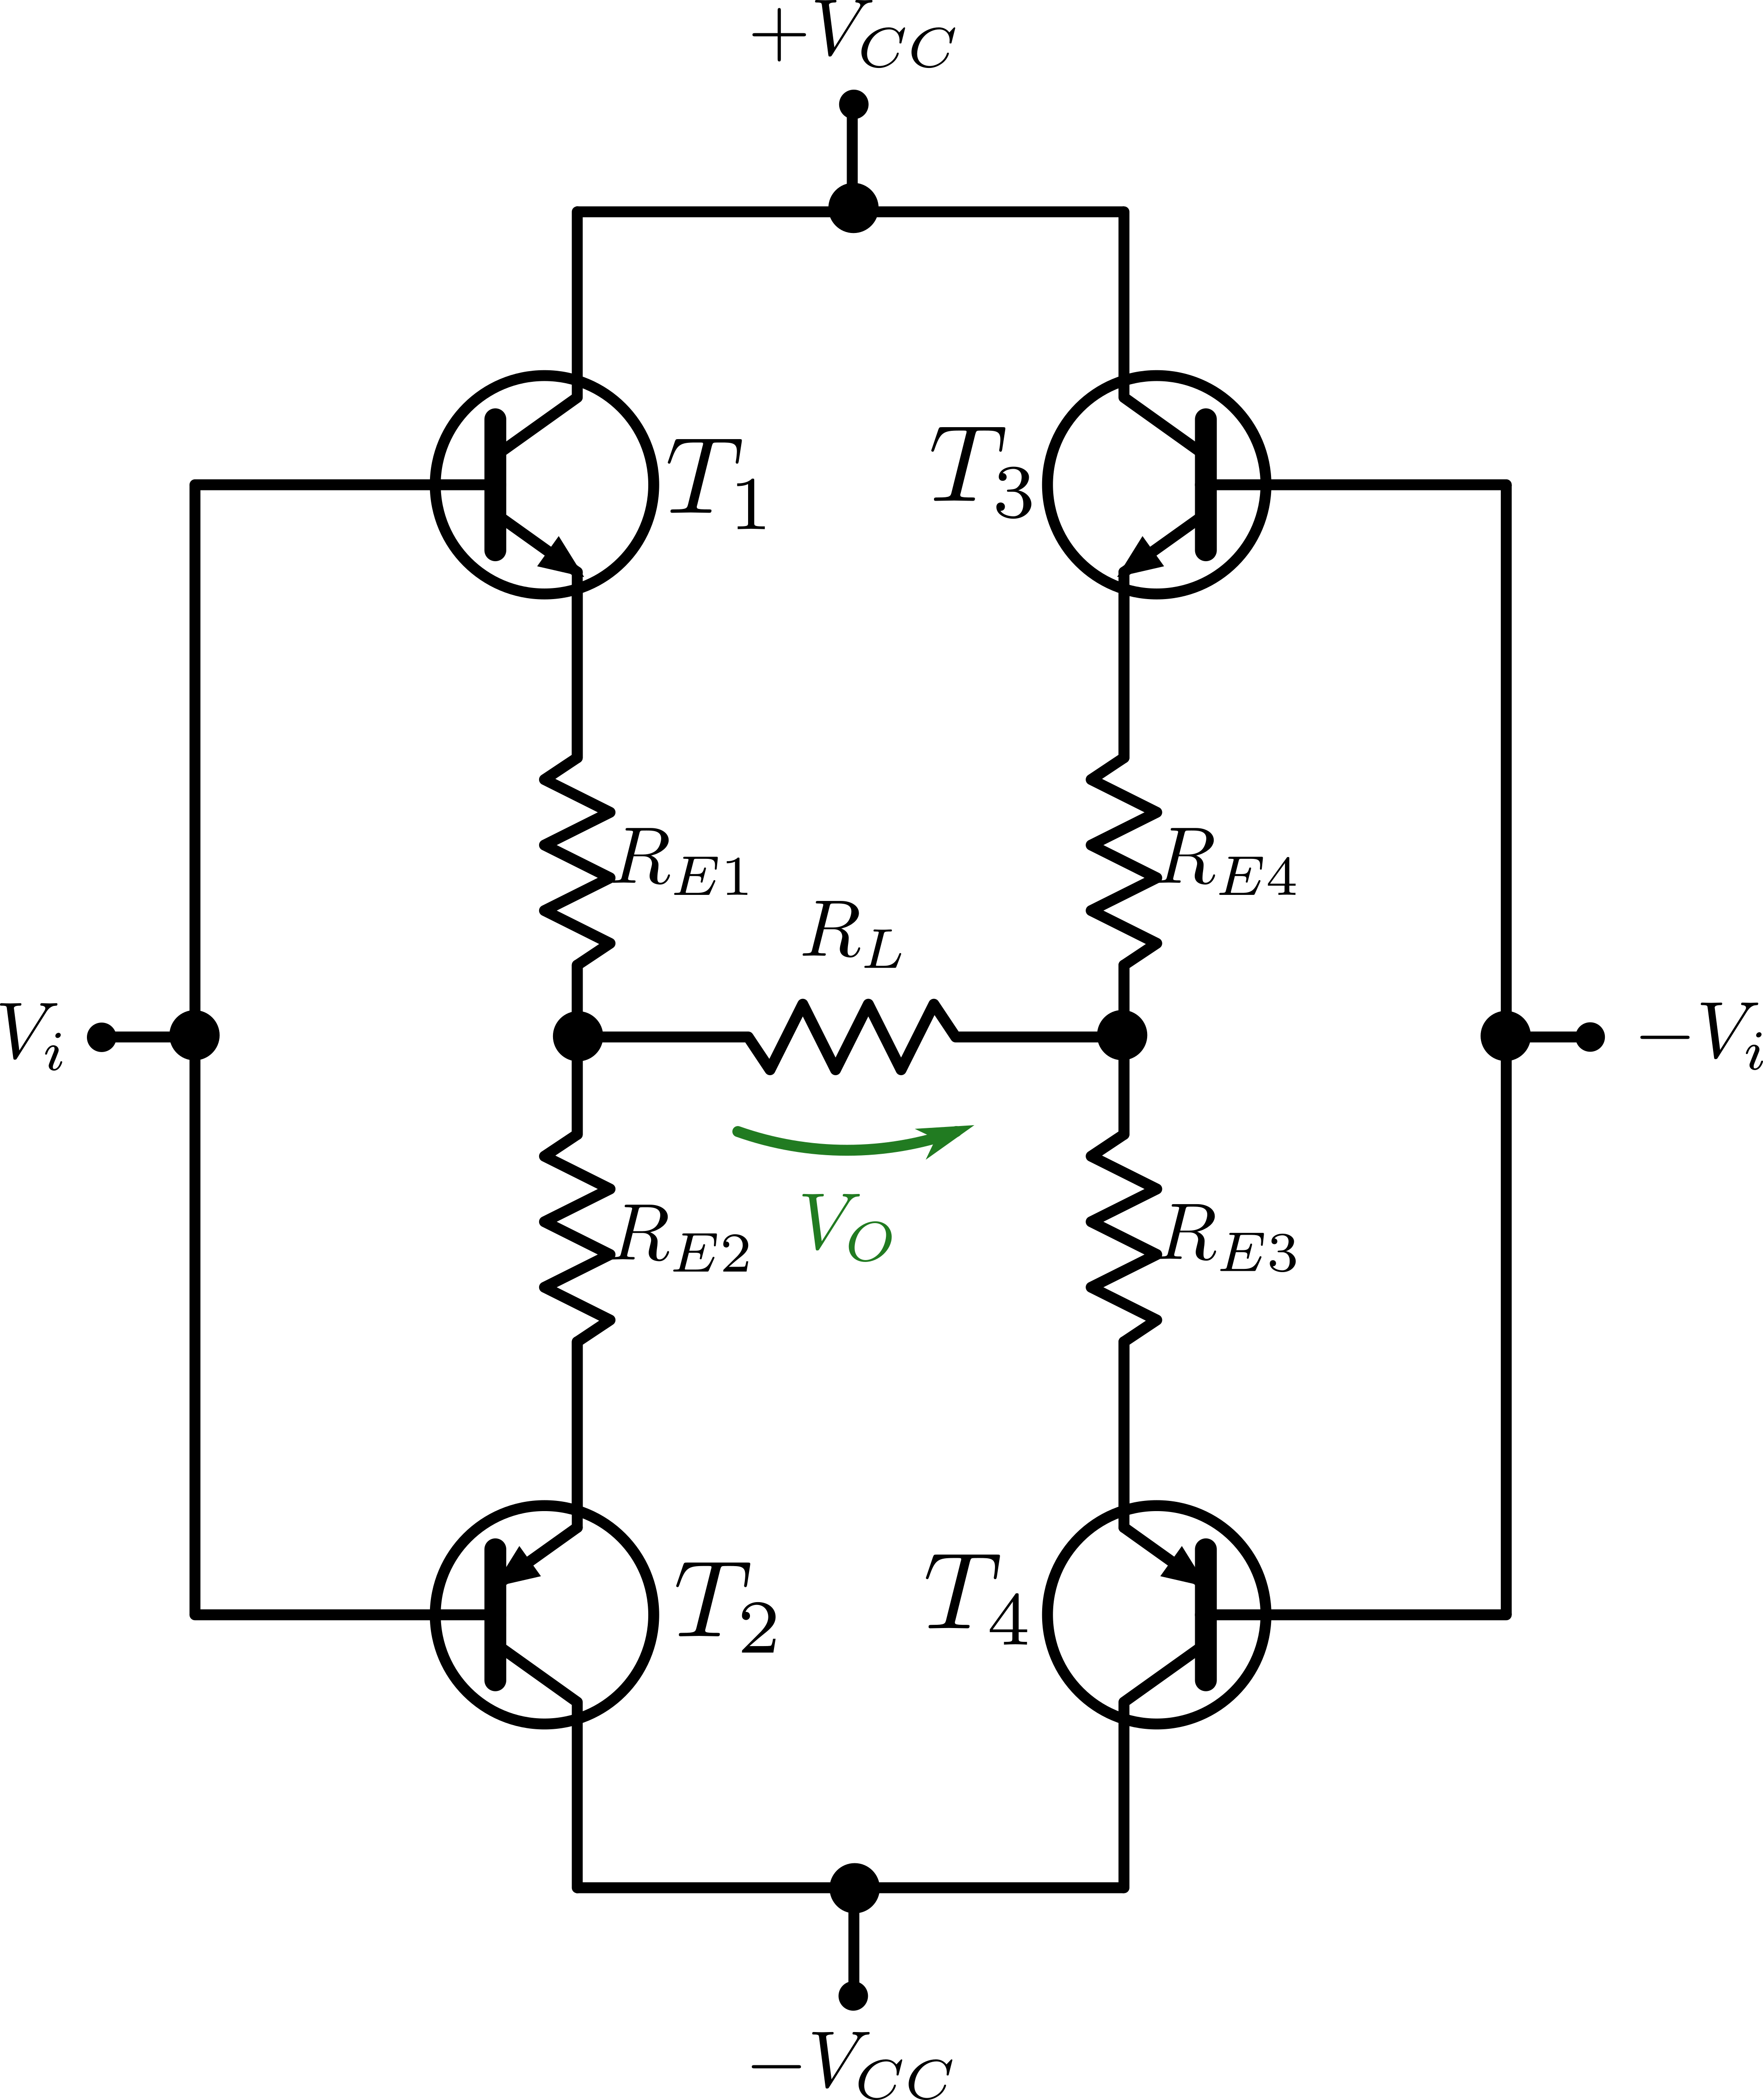
\includegraphics[scale=0.5]{Imagenes/EtapaSalida.png}
\par\end{centering}
\caption{Etapa de salida diferencial}
\end{figure}

Teniendo la potencia buscada sobre la carga, se puede realizar el diseño del amplificador desde ``afuera hacia adentro'' (es decir, desde la salida hacia el generador de entrada).\par
Siendo que se trabaja con señales senoidales, la potencia de salida que se toma en cuenta es la potencia eficaz, teniendo:

\[
P_{O_{MAX}} = \frac{V_{O_{RMS}}}{R_L} = \frac{{\hat{V_O}_{MAX}}^2}{2 \cdot R_L}
\]

Considerando para el diseño que $P_{O_{MAX}} = 25W$, se calcula la $\hat{V_O}_{MAX}$ necesaria:

\[
P_{O_{MAX}} = \frac{{\hat{V_O}_{MAX}}^2}{2 \cdot R_L} \Longrightarrow \hat{V_O}_{MAX} = \sqrt{2 \cdot R_L \cdot P_{O_{MAX}}} = 20V
\] 

Dicha tensión sería la tensión pico máxima diferencial sobre la carga. Tomando uno de sus bornes respecto de masa, es la mitad del valor, es decir $\frac{\hat{V_O}_{MAX}}{2} = 10V$.\par
Con la tensión calculada, se puede obtener la $\hat{I_O}_{MAX}$ sobre la carga:

\[
\hat{I_O}_{MAX} = \frac{\hat{V_O}_{MAX}}{R_L} = 2.5A
\]

Unos transistores de potencia adecuados a estas especificaciones son los darlington complementarios TIP122 (NPN) y TIP127 (PNP). Por lo que se seleccionan $T_1 = T_3 = \textrm{TIP122}$ y $T_2 = T_4 = \textrm{TIP127}$.\par
Las resistencias $R_{E1}$, $R_{E2}$ $R_{E3}$ y $R_{E4}$ se colocan para evitar que los transistores se quemen debido al efecto que se conoce como ``embalamiento térmico''. Esto se explica más en detalle junto con el efecto de distorsión por cruce por cero en la sección sobre prepolariación.

%FALTA REVISAR LA EXPLIACION ESTA!!!

Esta implementación presenta algunas ventajas respecto de una con salida referida a masa. En el caso de este último (correspondería tomar solo una de las dos mitades del circuito), cada fuente de alimentación aporta corriente en uno de los dos semiciclos de señal (dado que en cada semiciclo conduce solo uno de los dos transistores NPN o PNP), mientras que en la implementación propuesta ambas fuentes proporcionan corriente en ambos semiciclos. En el semiciclo positivo (es decir, tomando $V_i > 0$) conducen los transistores $T_1$ y $T_4$, mientras que en el negativo conducen $T_2$ y $T_3$. Esta configuración es conocida como ``Puente H'', la cual es común implementarla en el control de sentido de giro de un motor (siendo el motor la carga $R_L$).\par
Se considera nuevamente:

\[
P_{O_{MAX}} = \frac{{\hat{V_O}_{MAX}}^2}{2 \cdot R_L}
\]

Para observar una de las ventajas de esta implementación, se toma medio circuito (como se mencionó anteriormente), diseñándolo para una cierta potencia $P_{O_{MAX}}$, que dará lugar a una $\hat{V_O}_{MAX}$. El otro hemicircuito será similar pero con una fase de $180^{\circ}$. Conectando la carga $R_L$ entre ambas salidas, en cada terminal de la misma se tendría entonces $V_O$ y $-V_O$ respectivamente. Esto quiere decir que sobre la carga se tendría una diferencia de tensión de $2V_O$. Si se reemplaza en la ecuación de potencia anterior, resulta que la $P_{O_{MAX}}$ en el circuito propuesto es cuatro veces mayor que para el mismo diseño sobre un circuito con salida referida a masa, utilizando fuentes de alimentación de igual valor de tensión en ambos casos (pero las fuentes deberán ser del doble de potencia para el circuito diferencial).\par
Se detalla el cálculo de las potencias en la sección de cálculo de protección térmica con disipador.

\subsection{Prepolarización}

%EFECTO DE CRUCE POR CERO Y EMBALAMIENTO TERMICO

\subsection{Fuente de corriente $I_F$}

Para las fuentes de corriente $I_F$ expresadas en el diseño, se implementó el siguiente circuito:

\begin{figure}[!ht]
\begin{centering}
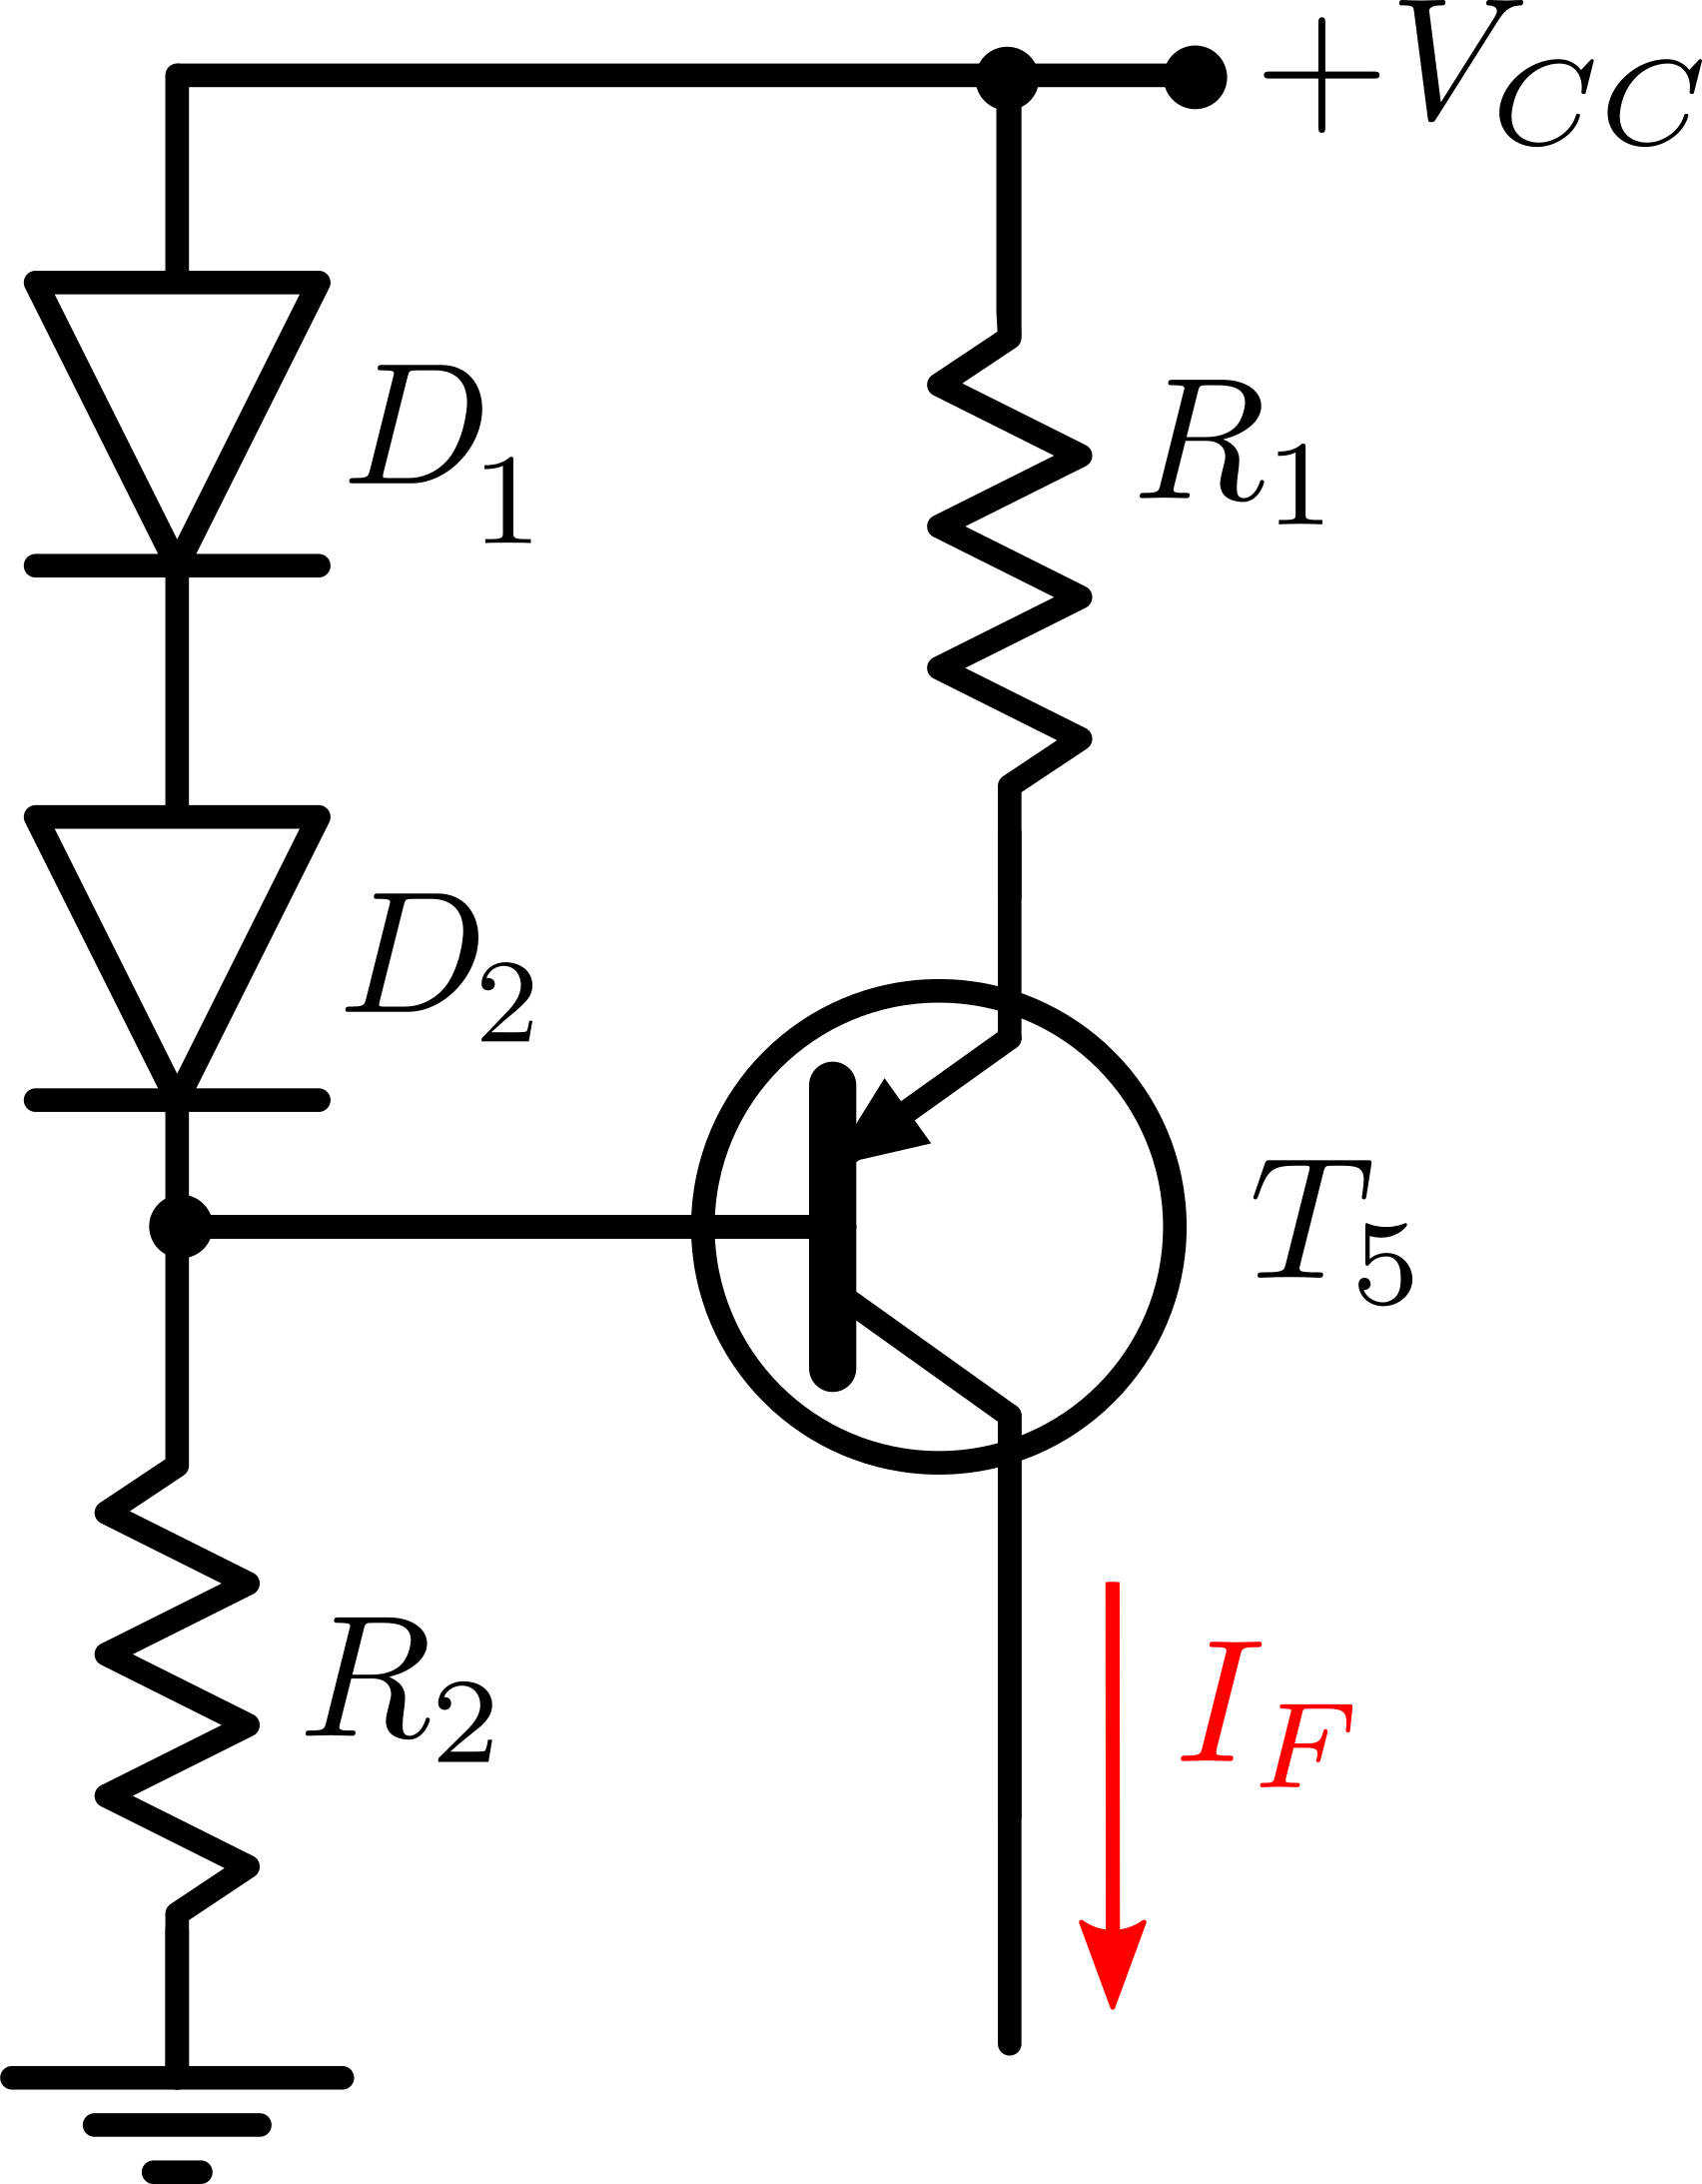
\includegraphics[scale=0.5]{Imagenes/FuenteIF.png}
\par\end{centering}
\caption{Fuente de corriente}
\end{figure}

Dado que la función de los diodos $D_1$ y $D_2$ es solamente provocar una caída de tensión similar a la $V_{EB5_{ON}}$, se utilizan los comunes 1N4148. Considerando que $R_2$ permite polarizarlos correctamente, se tiene recorriendo la malla:

\[
V_{D2} + V_{D1} - I_F \cdot R_1 - V_{EB5_{ON}} = 0
\]

Considerando $V_{D1} = V_{D2} = V_{EB5_{ON}} = V_D = 0.7V$, se tiene:

\[
I_F \cdot R_1 = V_D \Longrightarrow R_1 = \frac{V_D}{I_F}
\]

Del diseño de la etapa de potencia se obtuvo que $\hat{I_O}_{MAX} = 2.5A$. Considerando que los transistores TIP utilizados poseen un $HFE_{MIN} = 1000$ según la hoja de datos (ON Semiconductor), se calcula la corriente de base mínima necesaria que deberá poder proveerles la fuente de corriente (tomando de referencia al transistor $T_1$):

\[
\left. I_{B1_{MIN}} \right|_{I_{O_{MAX}}} = \frac{\hat{I_O}_{MAX}}{HFE_{MIN}} = 2.5mA \Longrightarrow I_{F_{MIN}} = 2.5mA
\]

Entonces se tiene:

\[
R_{1_{MAX}} = \frac{V_D}{I_{F_{MIN}}} = 280\Omega \Longrightarrow R_1(N) = 270\Omega
\]

Se normaliza hacia abajo para asegurar la $I_{F_{MIN}}$.\par
Teniendo ya la etapa de potencia y la fuente de corriente diseñadas, se puede determinar la $V_{CC_{MIN}}$ de acuerdo al camino formado desde la carga, pasando por $R_{E1}$, $T_1$ (como referencia tomando el semiciclo positivo), $T_5$ y $R_1$. Recordando que en un borne de la carga respecto a masa se tiene en el peor caso $\frac{\hat{V_O}_{MAX}}{2}$:

\[
\frac{\hat{V_O}_{MAX}}{2} + \hat{I_O}_{MAX} \cdot R_{E1} + V_{BE1_{ON}} + V_{EC5_{SAT}} + V_D = V_{CC_{MIN}} \Longrightarrow V_{CC_{MIN}} = 13.625V
\]

Como fuente normalizada se utilizará $V_{CC} = \pm 15V$, para asegurar dichas tensiones en el peor caso, considerando además que la tensión que entrega la fuente puede caer un pequeño porcentaje al trabajar con la carga a potencia máxima.\par
Con la fuente de tensión definida, se puede calcular ahora $R_2$ de manera de asegurar la polarización de los diodos. Tomando una corriente en directa $I_D$ para los diodos 1N4148 de 2mA, se tiene (despreciando la corriente de base de $T_5$):

\[
V_{CC} - 2 \cdot V_D - I_D \cdot R_2 = 0
\]

\[
 R_{2_{MAX}} = \frac{V_{CC} - 2 \cdot V_D}{I_D} = 6.8K\Omega \Longrightarrow R_2(N) = 4.7K\Omega
\]

Normalizando hacia abajo de manera tal de asegurar la $I_D$.\par
Dado que no hay requerimientos particulares de corriente o tensión sobre $T_5$, se utiliza de los disponibles el BC327.\par
Para la fuente de corriente del otro hemicircuito, los componentes son idénticos.

\subsection{Etapa de ganancia de tensión}

Para la etapa de ganancia de tensión, se utiliza un amplificador operacional en configuración no inversor. El integrado utilizado es el TL084, de los más comunes utilizados en audio, dada su baja distorsión armónica y alta impedancia de entrada. El circuito en cuestión es el siguiente.

\begin{figure}[!ht]
\begin{centering}
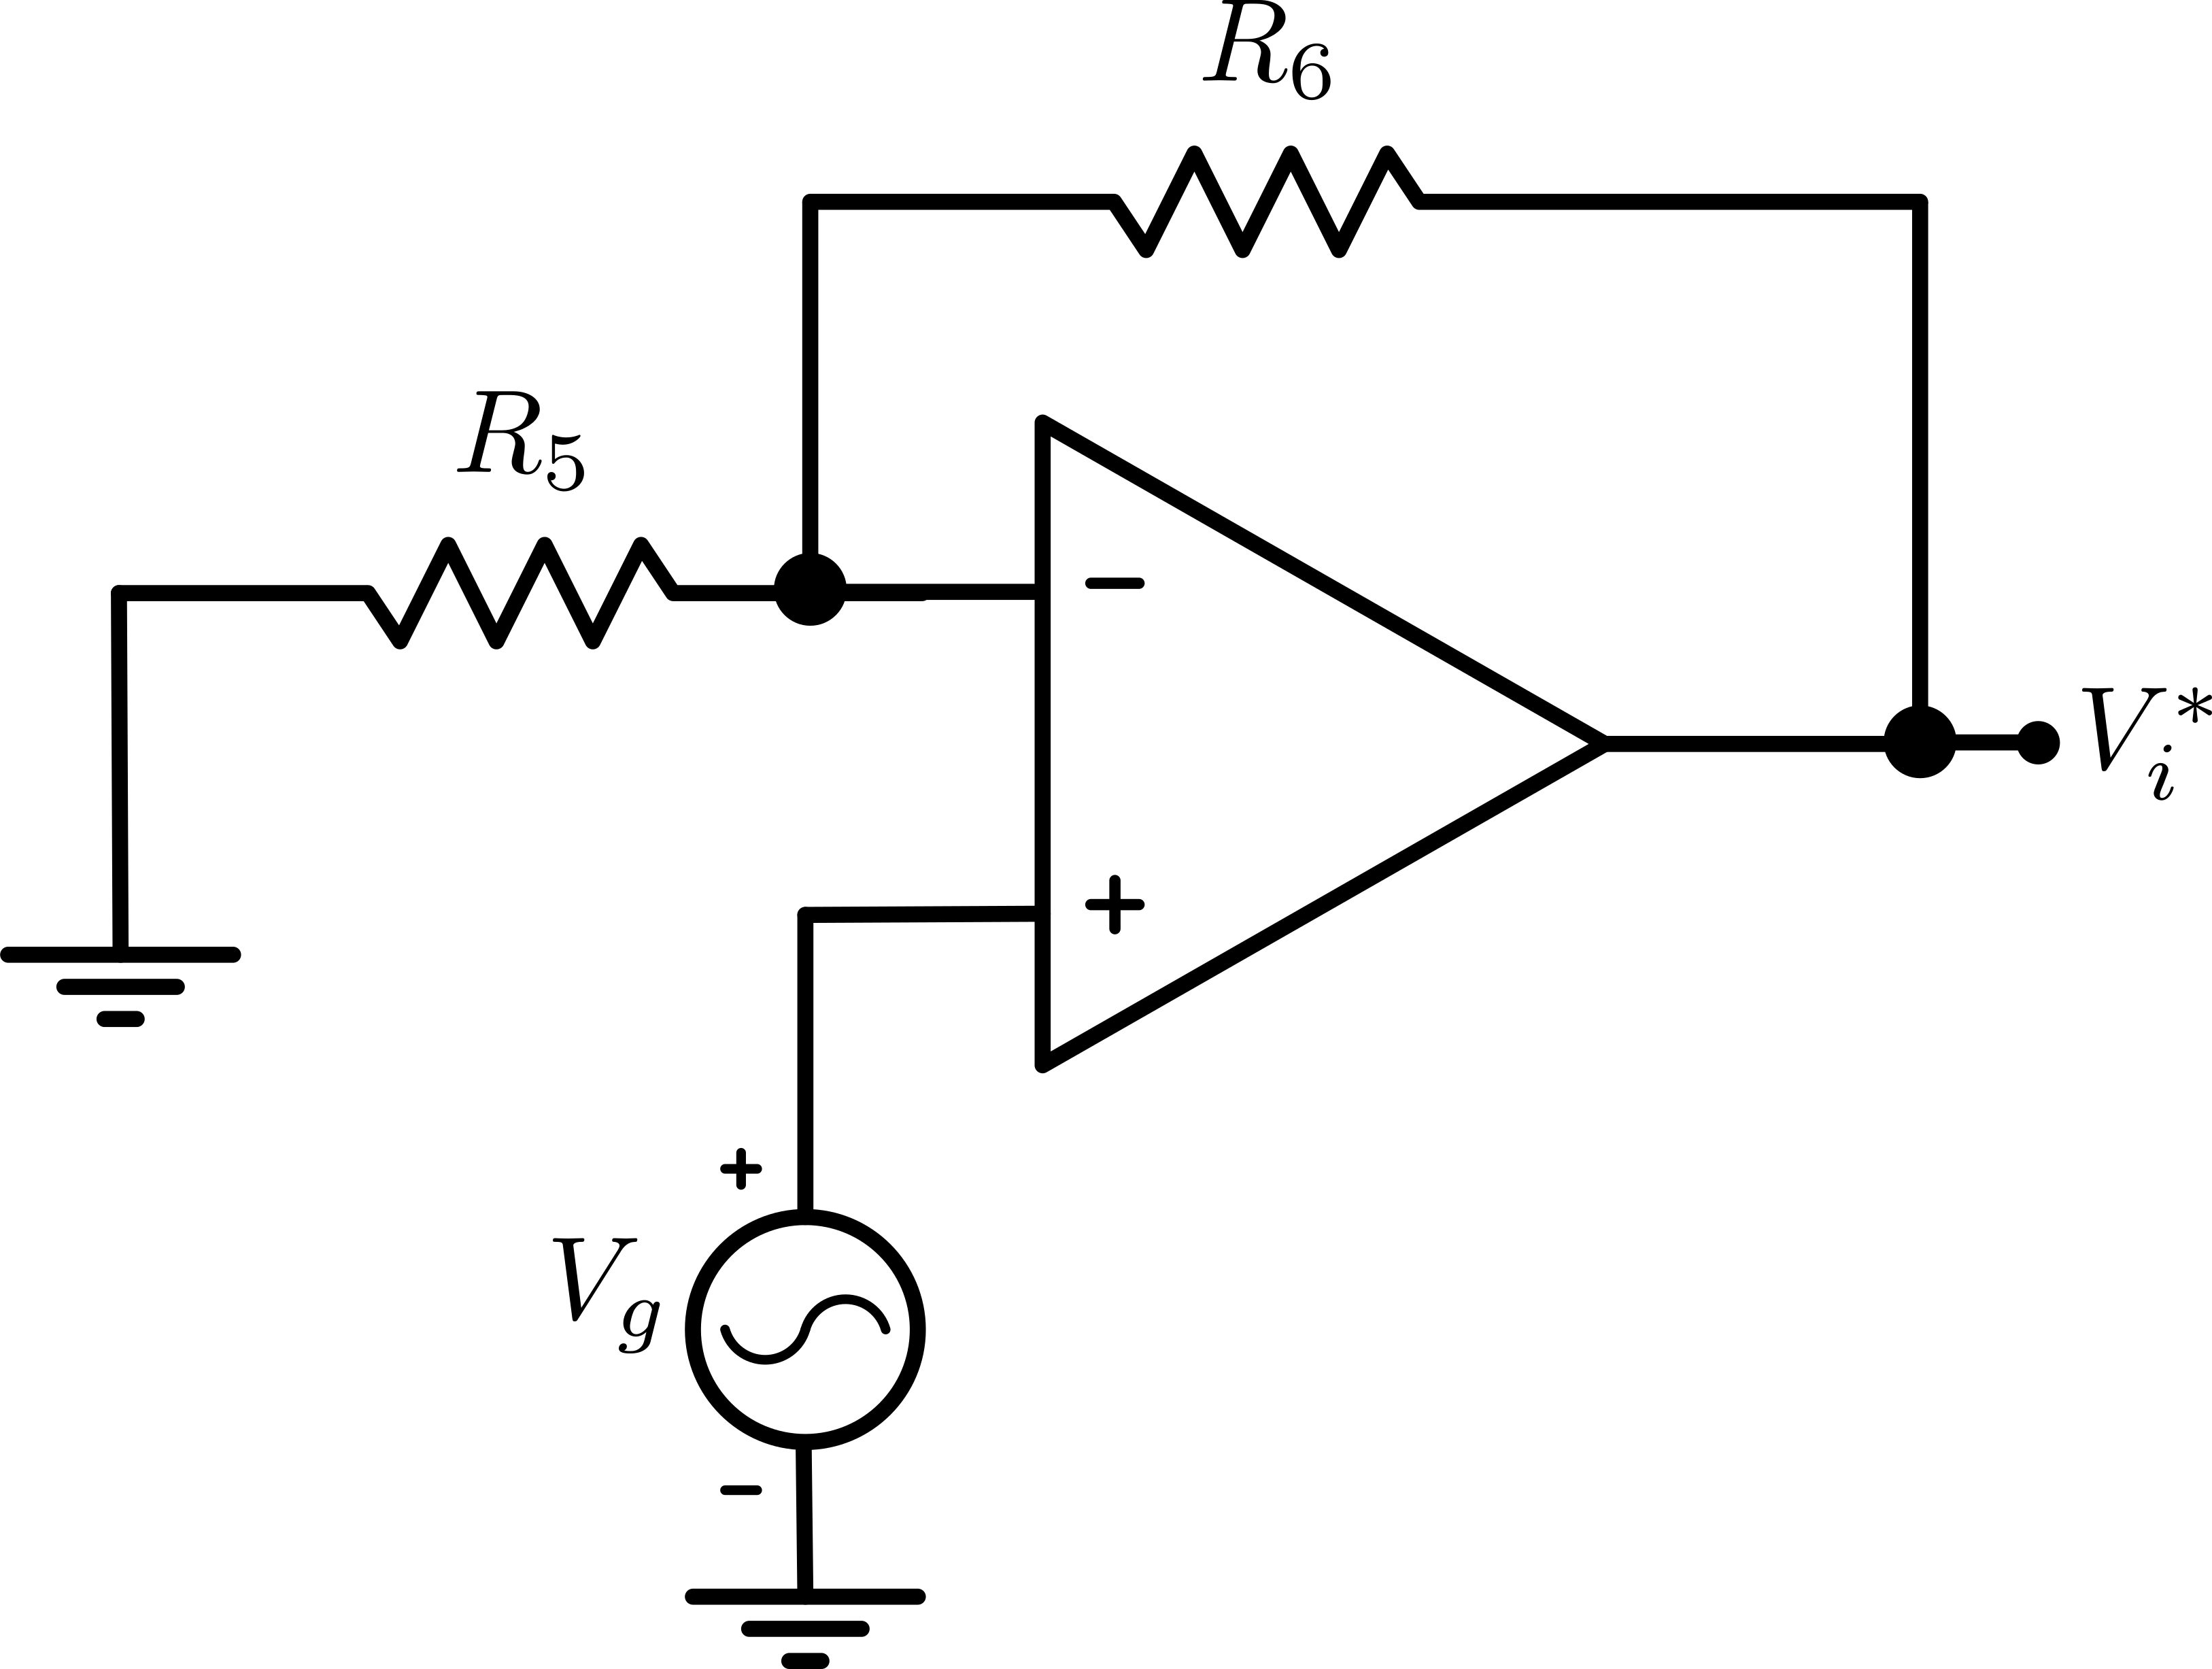
\includegraphics[scale=0.5]{Imagenes/EtapaDeAV.png}
\par\end{centering}
\caption{Amplificador de tensión}
\end{figure}

Dado que la etapa de salida es colector común, se aproxima su ganancia de tensión como unitaria por simplicidad. Sabiendo entonces que se da como parámetro que para la máxima potencia de salida, la señal de entrada es $\hat{V_g}_{MAX} = 0.5V$, y que en cualquiera de los bornes de la carga se tiene en dicho caso $\frac{\hat{V_O}_{MAX}}{2} = 10V$ respecto de masa, la ganancia de tensión necesaria es de:

\[
A_V = \frac{V_i^*}{V_g} = \frac{ \frac{\hat{V_O}_{MAX}}{2} }{\hat{V_g}_{MAX}} = 20
\]

De la expresión conocida para la ganancia de tensión del no inversor:

\[
A_V = \left( 1 + \frac{R_6}{R_5} \right) = 20
\]

Se toman $R_5(N) = 10K\Omega$, y $R_6(N) = 180K\Omega + 10K\Omega$ (serie).

Para producir la señal invertida para el otro hemicircuito, se toma la salida $V_i^*$ de esta etapa y se conecta a otro amplificador operacional en configuración inversora de ganancia de tensión -1. En la figura se muestra como queda dicho conjunto.

\begin{figure}[!ht]
\begin{centering}
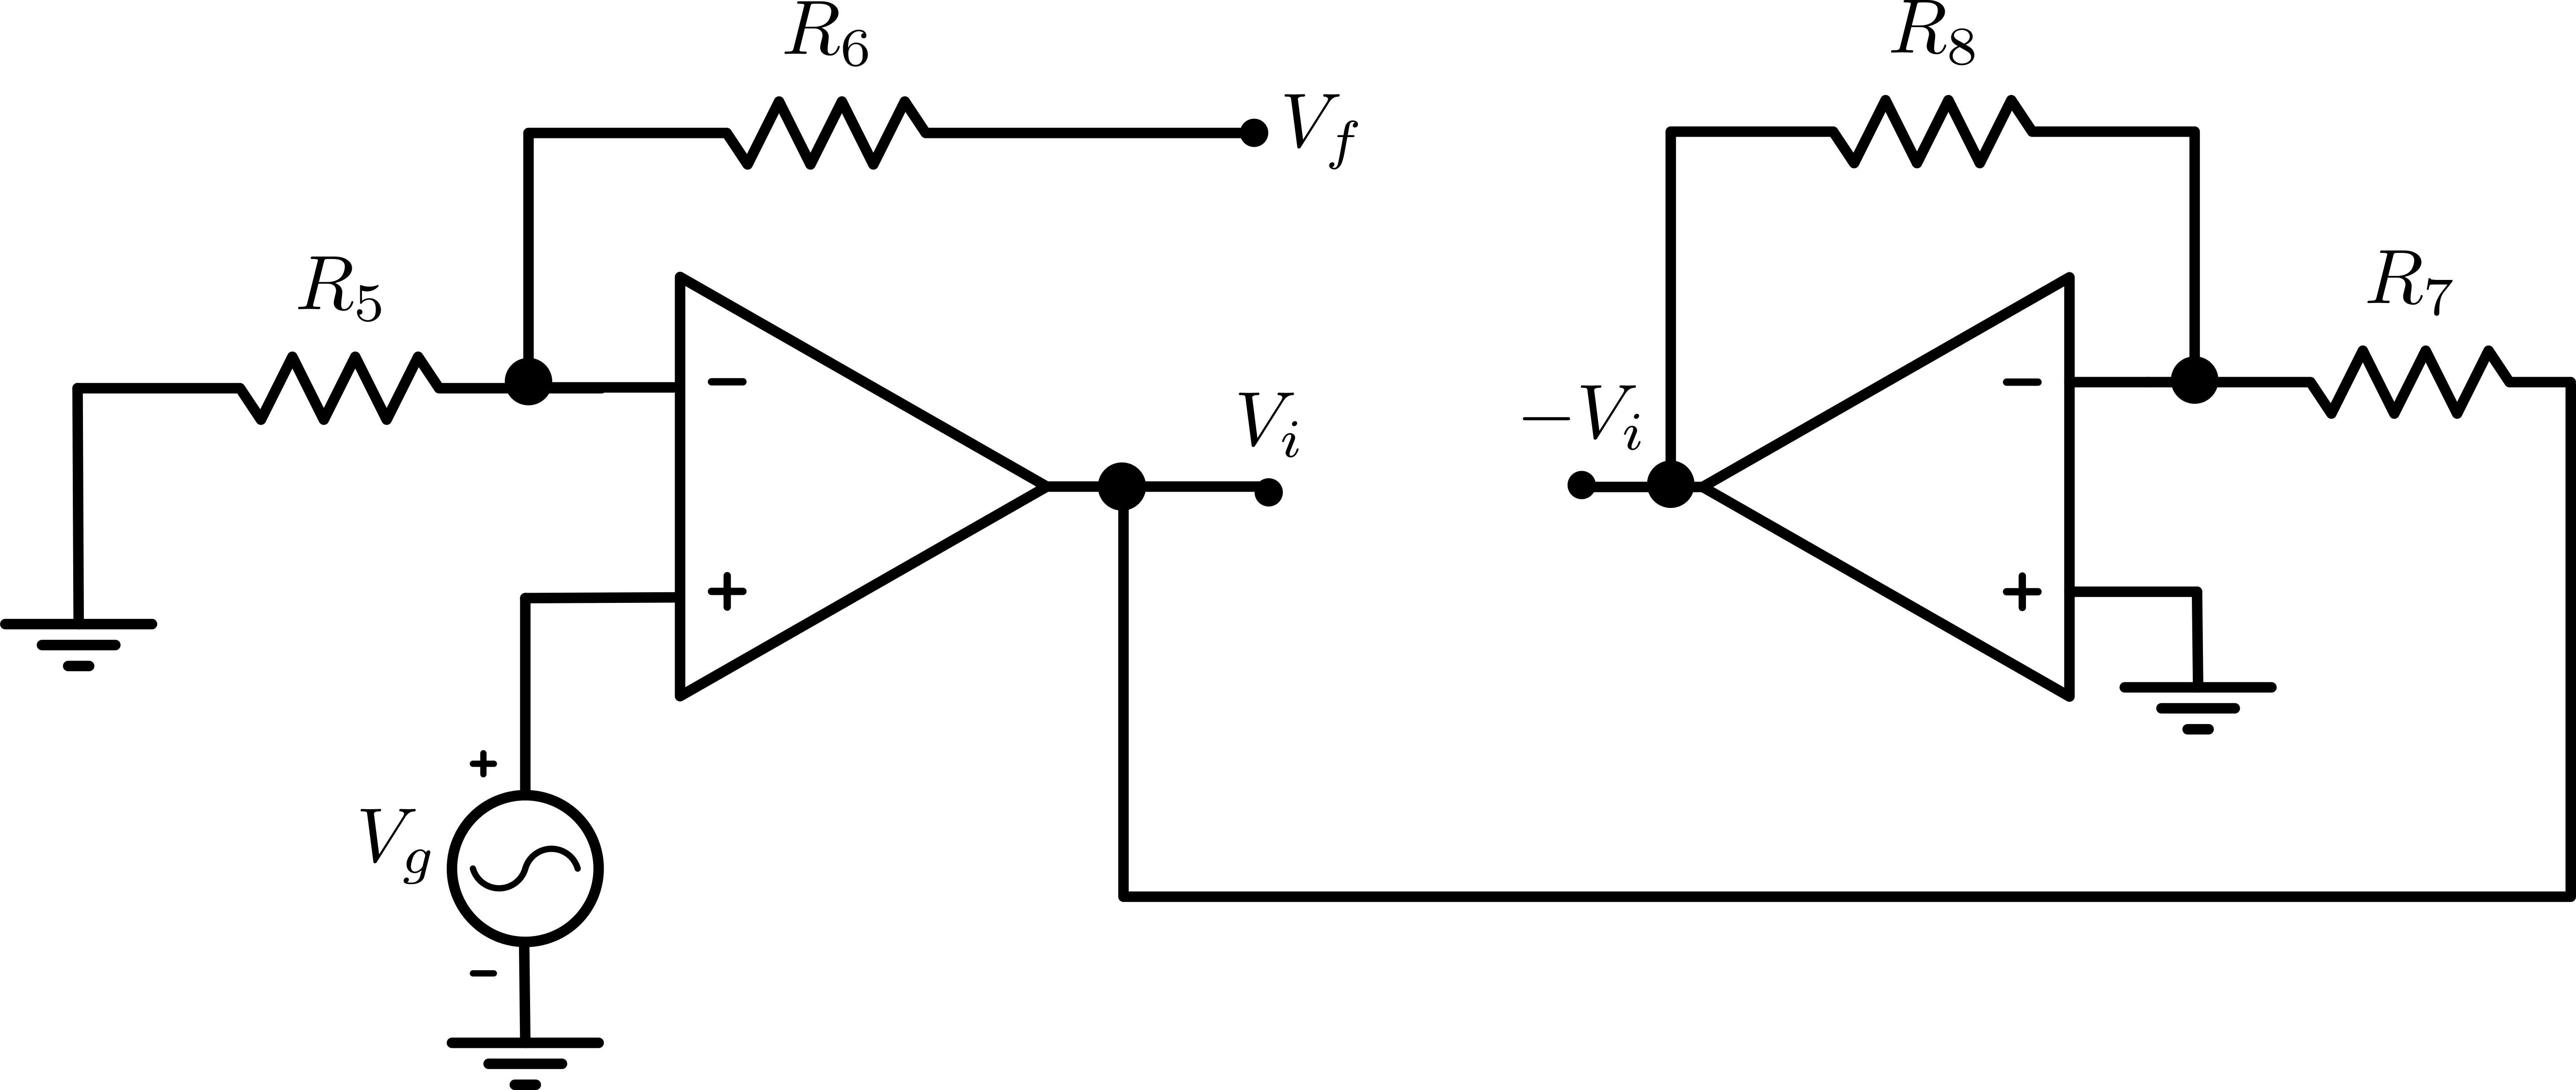
\includegraphics[scale=0.5]{Imagenes/opamp2SinCap.png}
\par\end{centering}
\caption{Amplificador de tensión e inversión de señal}
\end{figure}

En la figura se hace una distinción particular con $V_f$, dado que la ganancia se calculó tomando como tensión que muestrea el lazo como $\frac{\hat{V_O}_{MAX}}{2}$. Como la señal a muestrear debe ser la salida del circuito y ésta es diferencial, se debe tomar dicha salida y hacer la diferencia propiamente dicha, dividida por 2. Es decir:

\[
V_f = \frac{1}{2}\left( \frac{\hat{V_O}_{MAX}}{2} - \left( -\frac{\hat{V_O}_{MAX}}{2} \right) \right) = \frac{\hat{V_O}_{MAX}}{2}
\]

De esta manera, la señal muestreada resultante $V_f$ es la llamada en el primer circuito como $V_i^*$.

\subsubsection{Reestricción del ancho de banda}

%LOS CALCULOS PARA LOS CAPACITORES DE 20KHZ Y 20HZ

\end{document}
